\documentclass[t]{beamer}

% Load general definitions
% Preamble file - general definitions, package loading, etc.

%=================================
% Load packages
\usepackage{amssymb,amsmath}
\usepackage{graphicx}
\usepackage{url}
\usepackage{tikz}
\usetikzlibrary{mindmap,trees,arrows}
\usepackage{fancyvrb}
\usepackage[portuguese]{babel} 
\usepackage[utf8]{inputenc}
\usepackage{subfigure}
\usepackage{times}
\usepackage[T1]{fontenc}
\usepackage{cancel}
\usepackage{color}
\usepackage{listings}
\usepackage[document]{ragged2e}

%=================================
% Set mode
\mode<presentation>
{
	\usetheme{Madrid}
	\usecolortheme{structure}
	\useoutertheme{infolines}
	\setbeamercovered{invisible}
}

% Get rid of nav bar
\beamertemplatenavigationsymbolsempty

% Insert frame number at bottom of the page.
\usefoottemplate{\hfil\tiny{\color{black!90}\insertframenumber}} 

%=================================
% Define new commands

\newcommand\Real{{\mathbb{R}}}
%\newcommand{\vi}{\vspace{0.6\baselineskip}}
%\newcommand{\goodgap}{\hspace{\subfigtopskip}\hspace{\subfigbottomskip}}


% Equation environments
\newcommand{\beq}{\begin{equation}}
\newcommand{\eq}{\end{equation}}
\newcommand{\beqs}{\begin{equation*}}
\newcommand{\eqs}{\end{equation*}}
\newcommand{\beqn}{\begin{eqnarray}}
\newcommand{\eqn}{\end{eqnarray}}
% Bold variables
\newcommand{\mbf}[1]{\ensuremath{\mathbf{#1}}}
% Itemization
\newcommand{\bitem}{\begin{itemize}}
\newcommand{\eitem}{\end{itemize}}
\newcommand{\spitem}{\vskip 1em\item}
\newcommand{\bitems}{\begin{itemize}\item}
\newcommand{\benums}{\begin{enumerate}\item}
\newcommand{\eenum}{\end{enumerate}}
% color blocks
\newenvironment{colorblock}[2]{%
\setbeamercolor{block title}{#2}
\begin{block}{#1}}{\end{block}}
% Vertical spacing
\newcommand{\vone}{\vskip 1em}
\newcommand{\vhalf}{\vskip .5em}
% Frame environments
\newenvironment{ftst}[3][t]{%
\begin{frame}{environment=ftst,#1}
\frametitle{#2}
\framesubtitle{#3}}{\end{frame}}
\newenvironment{ftstf}[2]{
\begin{frame}[fragile,environment=ftstf]
\frametitle{#1}
\framesubtitle{#2}}{\end{frame}}
% colors
\definecolor{MyGray}{rgb}{0.5,0.5,0.5}
\definecolor{MyDBGray}{rgb}{0.1,0.1,0.4}
\definecolor{darkgreen}{rgb}{0,0.4,0}
\definecolor{black}{rgb}{0,0,0}
\def\defn#1{{\color{red} #1}}
% Footnote
\renewcommand{\thefootnote}{\alph{footnote}}
% Relaxed footnotes
\newcommand{\lfr}[1]{\let\thefootnote\relax\footnote{\tiny #1}}
% Verbatim environment - using FANCYVRB package
\DefineVerbatimEnvironment%
{rcode}{Verbatim}
{fontsize=\scriptsize}
% Verbatim environment - using LISTINGS package
%\lstnewenvironment{rcode} {\lstset{	language = R,
%									basicstyle = \scriptsize\ttfamily,
%									showspaces = false,
%									showstringspaces = false,
%									showtabs = false,
%									keywordstyle = \color{black}\bfseries,
%									commentstyle = \color{darkgreen},
%									numbers = none,
%									otherkeywords={	<-,
%													ggplot,
%													geom_boxplot,
%													facet_grid,
%													shapiro.test,
%													fligner.test,
%													glht,
%													with},
%									deletekeywords={data,
%													model,
%													residuals,
%													c,
%													axis,
%													default,
%													labels,
%													qq.text}}}%
%{}

% Specific definitions
\title[]{Algoritmos e Estruturas de Dados III}
\subtitle[]{Caminhos Euleriano e Hamiltoniano}
\author[]{Patrícia Lucas\\{\footnotesize }}
\institute{Bacharelado em Sistemas de Informação \\ IFNMG  - Campus Salinas}
\date{\scriptsize Salinas\\Dezembro 2020}

\begin{document}

% cover page
\setbeamertemplate{footline}{}
\begin{frame}

\begin{center}
\includegraphics[width=.15\textwidth]{}
\end{center}
  \titlepage
  \begin{tikzpicture}[remember picture,overlay]
  \node[anchor=south east,xshift=-5pt,yshift=5pt] at (current page.south east) {\tiny Versão 1.2020};
  \node[anchor=south west,yshift=0pt] at (current page.south west) {
\includegraphics[width=.25\textwidth]{Logos/salinas_horizontal_jpg.jpg}};
  \end{tikzpicture}  
\end{frame}


%=====

% Main slides
\begin{ftst}{Caminhos Eulerianos}{História}
\vone
\vone
\begin{minipage}{.5\textwidth}
    \centering
    \justifying
    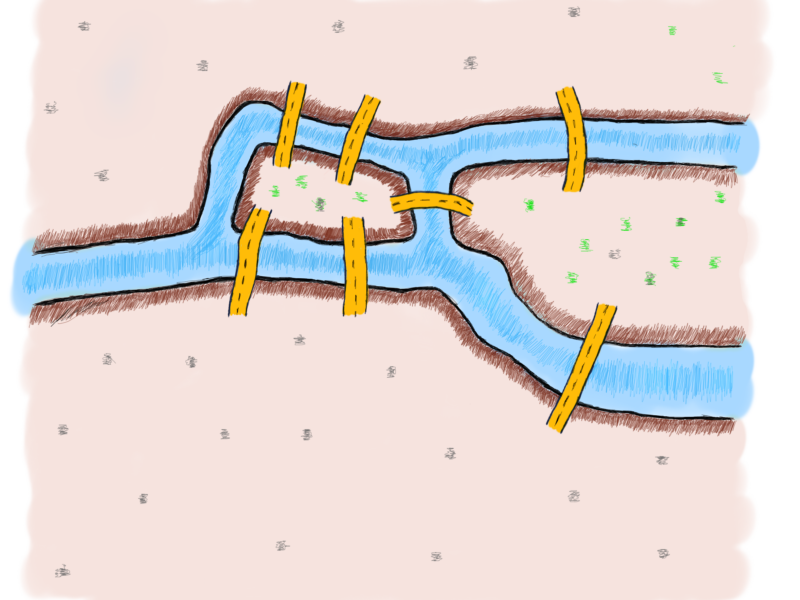
\includegraphics[scale=0.23]{Figuras/euleriano_1.png}
\end{minipage}%
\hfill
\begin{minipage}{.5\textwidth}
    \footnotesize
    \justifying
    \begin{itemize}
        \item Havia sete pontes em Königsberg conectando duas grandes ilhas cercadas pelo rio Prególia e duas porções de continentes divididas pelo mesmo rio.
        \item O problema ou apenas um quebra-cabeças com as pontes de Königsberg era poder andar pela cidade atravessando todas as sete pontes apenas uma vez. 
        \item Não deve haver nenhuma ponte não cruzada.
        \item Não deve haver nenhuma ponte não cruzada.
    \end{itemize}
\end{minipage}%
\vone
\vone
\tiny
Fonte da imagem: \hypertarget{clique aqui.}{https://bit.ly/36sPR8J}
\end{ftst}

%=====

\begin{ftst}{Caminhos Eulerianos}{História}

\begin{minipage}{.5\textwidth}
    \vone
    \centering
    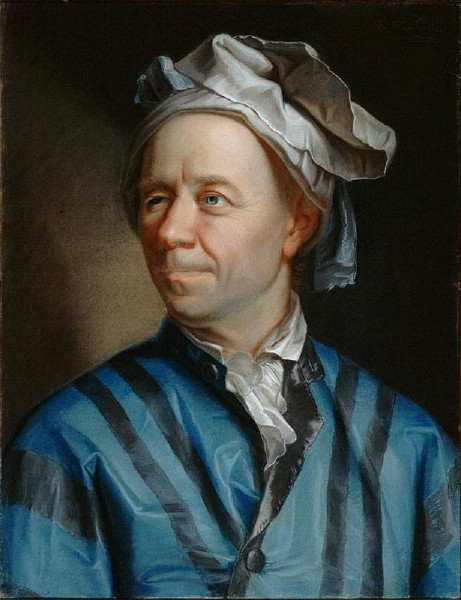
\includegraphics[scale=0.3]{Figuras/euler.jpeg}
\end{minipage}%
\hfill
\begin{minipage}{.5\textwidth}
    \justifying
    \footnotesize
    Às vezes é razoável desistir rapidamente. Foi assim que Euler resolveu esse problema - ele desistiu logo.
    \vone
    Em vez de tentar resolvê-lo, ele adotou uma abordagem diferente, tentando provar que não é possível andar pela cidade atravessando cada ponte uma única vez.
\end{minipage}
\vone
\tiny
Fonte da imagem: \hypertarget{clique aqui.}{https://bit.ly/36sPR8J}
\end{ftst}

%=====

\begin{ftst}{Caminhos Eulerianos}{História}
\vone
\vone
\begin{minipage}{.5\textwidth}
    \centering
    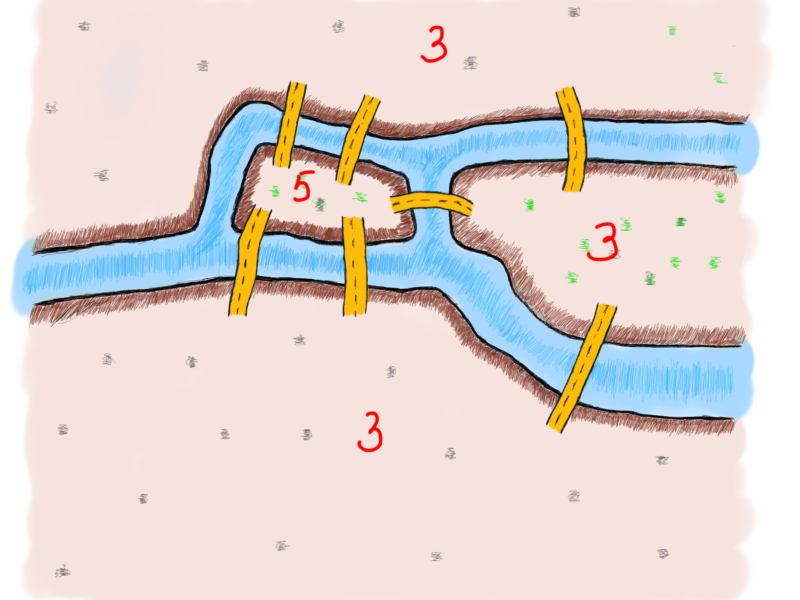
\includegraphics[scale=0.21]{Figuras/euleriano_2.png}
\end{minipage}%
\hfill
\begin{minipage}{.5\textwidth}
    \justifying
    \footnotesize
    Existem quatro lugares distintos: duas ilhas e duas partes do continente. 
    \vone
    Existem sete pontes interligando esses lugares. 
    \vone
    Padrões encontrados:
    \begin{itemize}
        \item Há um número ímpar de pontes conectadas a cada terra.
        \item Se você tiver que atravessar cada ponte uma vez, poderá entrar em um terreno e deixá-lo, se houver 2 pontes.
    \end{itemize}
\end{minipage}

\vone
\vone
\tiny
Fonte da imagem: \hypertarget{clique aqui.}{https://bit.ly/36sPR8J}
\end{ftst}

%=====

\begin{ftst}{Caminhos Eulerianos}{História}

Vamos adicionar uma nova ponte para ver como o número de pontes conectadas gerais muda e se resolve o problema.

\centering
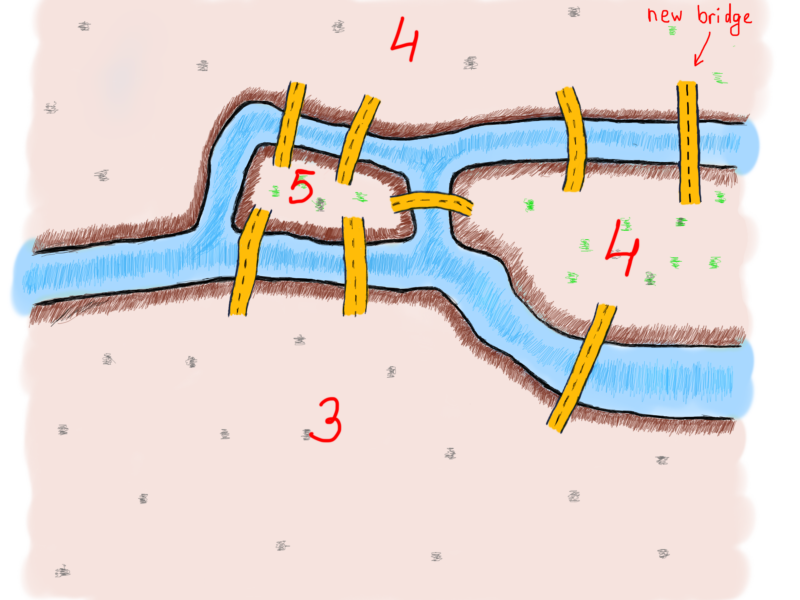
\includegraphics[scale=0.28]{Figuras/euleriano_6.png}

\justifying
\tiny
Fonte da imagem: \hypertarget{clique aqui.}{https://bit.ly/36sPR8J}
\end{ftst}

%=====

\begin{ftst}{Caminhos Eulerianos}{História}

Agora que temos dois pares (4 e 4) e dois ímpares (3 e 5) de pontes conectando os quatro pedaços de terra, vamos desenhar uma nova rota com a adição desta nova ponte.

\begin{minipage}{.5\textwidth}
    \centering
    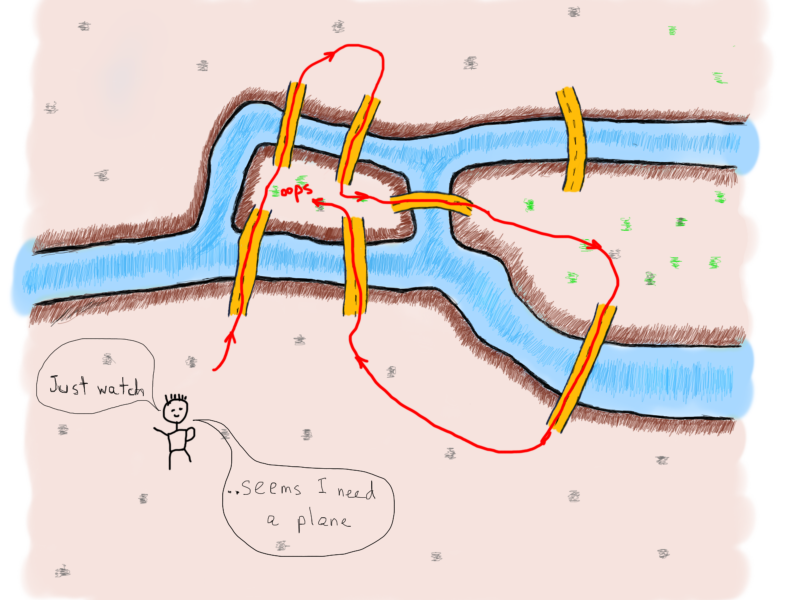
\includegraphics[scale=0.22]{Figuras/euleriano_3.png}
\end{minipage}%
\hfill
\begin{minipage}{.5\textwidth}
    \centering
    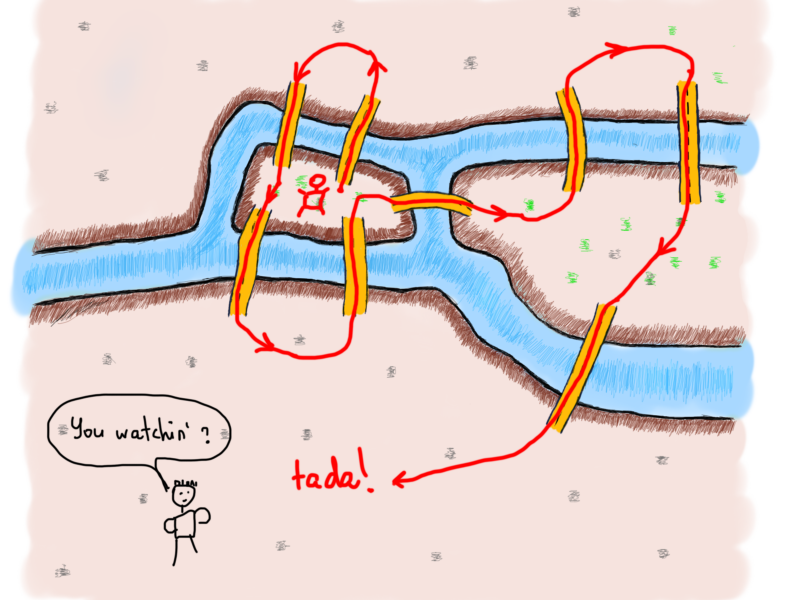
\includegraphics[scale=0.22]{Figuras/euleriano_4.png}
\end{minipage}

Ou seja, o número de pontes pares e ímpares determina se a solução é possível ou não.
\vone
\tiny
Fonte da imagem: \hypertarget{clique aqui.}{https://bit.ly/36sPR8J}
\end{ftst}

%=====

\begin{ftst}{Caminhos Eulerianos}{História}
\footnotesize
Foi quando Euler começou a "converter" terrenos e pontes em algo que conhecemos como grafos.

\centering
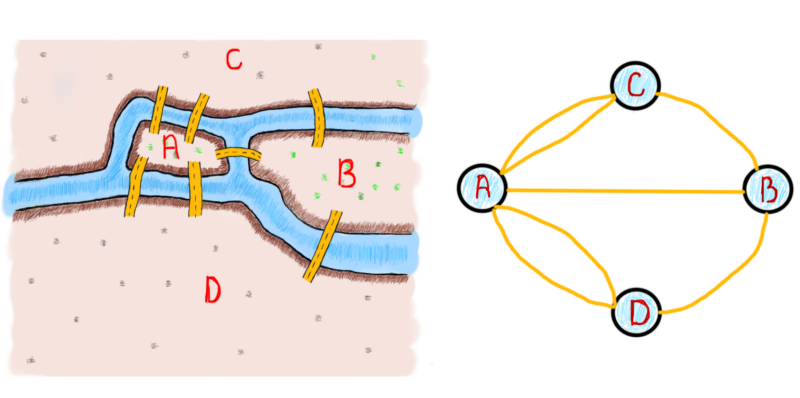
\includegraphics[scale=0.3]{Figuras/euleriano_5.png}

\justifying
\footnotesize
Euler mostrou que a possibilidade de um passeio pelo grafo (cidade) atravessando cada aresta (ponte) uma única vez depende estritamente dos graus dos vértices (terrenos). Esse caminho (em sua homenagem) ficou conhecido como \textbf{Caminho Euleriano}. \\
\vone
\tiny
Fonte da imagem: \hypertarget{clique aqui.}{https://bit.ly/36sPR8J}
\end{ftst}

%=====

\begin{ftst}{Caminhos Eulerianos}{Definições}

\begin{itemize}
    \item Um \textbf{caminho euleriano} é um caminho que passa exatamente uma vez por cada aresta de um grafo;
    \item Um \textbf{ciclo euleriano} é um caminho euleriano fechado, ou seja, começa e termina no mesmo vértice;
    \item Um \textbf{grafo euleriano} é um grafo que contém um ciclo euleriano;
    \item Um \textbf{grafo semi-euleriano} é um grafo que não contém um ciclo euleriano, mas contém um caminho euleriano.
\end{itemize}

\end{ftst}

%=====

\begin{ftst}{Grafo Euleriano}{Caminhos Eulerianos}
\vone
Um grafo conexo $G$ é um grafo euleriano se e somente se todos os seus vértices possuem grau par.
\vone
\centering


\tikzset{every picture/.style={line width=0.75pt}} %set default line width to 0.75pt        

\begin{tikzpicture}[x=0.75pt,y=0.75pt,yscale=-1,xscale=1]
%uncomment if require: \path (0,178); %set diagram left start at 0, and has height of 178

%Shape: Ellipse [id:dp4798267244017467] 
\draw  [draw opacity=0][fill={rgb, 255:red, 15; green, 118; blue, 237 }  ,fill opacity=1 ] (23.01,77.75) .. controls (23.01,73.74) and (26.33,70.48) .. (30.42,70.48) .. controls (34.51,70.48) and (37.83,73.74) .. (37.83,77.75) .. controls (37.83,81.77) and (34.51,85.02) .. (30.42,85.02) .. controls (26.33,85.02) and (23.01,81.77) .. (23.01,77.75) -- cycle ;
%Shape: Ellipse [id:dp44870182967820527] 
\draw  [draw opacity=0][fill={rgb, 255:red, 15; green, 118; blue, 237 }  ,fill opacity=1 ] (65.92,120.67) .. controls (65.92,116.66) and (69.24,113.41) .. (73.33,113.41) .. controls (77.42,113.41) and (80.74,116.66) .. (80.74,120.67) .. controls (80.74,124.69) and (77.42,127.94) .. (73.33,127.94) .. controls (69.24,127.94) and (65.92,124.69) .. (65.92,120.67) -- cycle ;
%Shape: Ellipse [id:dp6247177831364052] 
\draw  [draw opacity=0][fill={rgb, 255:red, 15; green, 118; blue, 237 }  ,fill opacity=1 ] (66.76,35.66) .. controls (66.76,31.64) and (70.08,28.39) .. (74.17,28.39) .. controls (78.26,28.39) and (81.58,31.64) .. (81.58,35.66) .. controls (81.58,39.67) and (78.26,42.93) .. (74.17,42.93) .. controls (70.08,42.93) and (66.76,39.67) .. (66.76,35.66) -- cycle ;
%Shape: Ellipse [id:dp24674115427755572] 
\draw  [draw opacity=0][fill={rgb, 255:red, 15; green, 118; blue, 237 }  ,fill opacity=1 ] (108.67,77.75) .. controls (108.67,73.74) and (111.99,70.48) .. (116.08,70.48) .. controls (120.17,70.48) and (123.49,73.74) .. (123.49,77.75) .. controls (123.49,81.77) and (120.17,85.02) .. (116.08,85.02) .. controls (111.99,85.02) and (108.67,81.77) .. (108.67,77.75) -- cycle ;
%Shape: Ellipse [id:dp24305715795512062] 
\draw  [draw opacity=0][fill={rgb, 255:red, 15; green, 118; blue, 237 }  ,fill opacity=1 ] (193.33,121.75) .. controls (193.33,117.74) and (196.65,114.48) .. (200.74,114.48) .. controls (204.83,114.48) and (208.15,117.74) .. (208.15,121.75) .. controls (208.15,125.77) and (204.83,129.02) .. (200.74,129.02) .. controls (196.65,129.02) and (193.33,125.77) .. (193.33,121.75) -- cycle ;
%Shape: Ellipse [id:dp44022017328235674] 
\draw  [draw opacity=0][fill={rgb, 255:red, 15; green, 118; blue, 237 }  ,fill opacity=1 ] (192.9,37.48) .. controls (192.9,33.47) and (196.22,30.21) .. (200.31,30.21) .. controls (204.4,30.21) and (207.72,33.47) .. (207.72,37.48) .. controls (207.72,41.5) and (204.4,44.75) .. (200.31,44.75) .. controls (196.22,44.75) and (192.9,41.5) .. (192.9,37.48) -- cycle ;
%Straight Lines [id:da7847946315938599] 
\draw [color={rgb, 255:red, 15; green, 118; blue, 237 }  ,draw opacity=1 ][fill={rgb, 255:red, 0; green, 0; blue, 0 }  ,fill opacity=1 ][line width=1.5]    (30.42,77.75) -- (64.47,43.29) ;
\draw [shift={(67.28,40.45)}, rotate = 494.65] [fill={rgb, 255:red, 15; green, 118; blue, 237 }  ,fill opacity=1 ][line width=0.08]  [draw opacity=0] (13.4,-6.43) -- (0,0) -- (13.4,6.44) -- (8.9,0) -- cycle    ;
%Straight Lines [id:da4535819051227774] 
\draw [color={rgb, 255:red, 15; green, 118; blue, 237 }  ,draw opacity=1 ][fill={rgb, 255:red, 0; green, 0; blue, 0 }  ,fill opacity=1 ][line width=1.5]    (107.75,68.66) -- (74.17,35.66) ;
\draw [shift={(110.61,71.46)}, rotate = 224.5] [fill={rgb, 255:red, 15; green, 118; blue, 237 }  ,fill opacity=1 ][line width=0.08]  [draw opacity=0] (13.4,-6.43) -- (0,0) -- (13.4,6.44) -- (8.9,0) -- cycle    ;
%Straight Lines [id:da9862797560803531] 
\draw [color={rgb, 255:red, 15; green, 118; blue, 237 }  ,draw opacity=1 ][fill={rgb, 255:red, 0; green, 0; blue, 0 }  ,fill opacity=1 ][line width=1.5]    (39.37,86.22) -- (73.33,120.67) ;
\draw [shift={(36.56,83.37)}, rotate = 45.41] [fill={rgb, 255:red, 15; green, 118; blue, 237 }  ,fill opacity=1 ][line width=0.08]  [draw opacity=0] (13.4,-6.43) -- (0,0) -- (13.4,6.44) -- (8.9,0) -- cycle    ;
%Straight Lines [id:da524977452131772] 
\draw [color={rgb, 255:red, 15; green, 118; blue, 237 }  ,draw opacity=1 ][fill={rgb, 255:red, 0; green, 0; blue, 0 }  ,fill opacity=1 ][line width=1.5]    (81.44,112.72) -- (116.08,77.75) ;
\draw [shift={(78.63,115.56)}, rotate = 314.73] [fill={rgb, 255:red, 15; green, 118; blue, 237 }  ,fill opacity=1 ][line width=0.08]  [draw opacity=0] (13.4,-6.43) -- (0,0) -- (13.4,6.44) -- (8.9,0) -- cycle    ;
%Straight Lines [id:da817738331686477] 
\draw [color={rgb, 255:red, 15; green, 118; blue, 237 }  ,draw opacity=1 ][fill={rgb, 255:red, 0; green, 0; blue, 0 }  ,fill opacity=1 ][line width=1.5]    (200.31,37.48) -- (200.72,110.48) ;
\draw [shift={(200.74,114.48)}, rotate = 269.68] [fill={rgb, 255:red, 15; green, 118; blue, 237 }  ,fill opacity=1 ][line width=0.08]  [draw opacity=0] (13.4,-6.43) -- (0,0) -- (13.4,6.44) -- (8.9,0) -- cycle    ;
%Straight Lines [id:da27880354700522414] 
\draw [color={rgb, 255:red, 15; green, 118; blue, 237 }  ,draw opacity=1 ][fill={rgb, 255:red, 0; green, 0; blue, 0 }  ,fill opacity=1 ][line width=1.5]    (200.74,121.75) -- (126.2,85.22) ;
\draw [shift={(122.61,83.46)}, rotate = 386.11] [fill={rgb, 255:red, 15; green, 118; blue, 237 }  ,fill opacity=1 ][line width=0.08]  [draw opacity=0] (13.4,-6.43) -- (0,0) -- (13.4,6.44) -- (8.9,0) -- cycle    ;
%Straight Lines [id:da7034873595191173] 
\draw [color={rgb, 255:red, 15; green, 118; blue, 237 }  ,draw opacity=1 ][fill={rgb, 255:red, 0; green, 0; blue, 0 }  ,fill opacity=1 ][line width=1.5]    (116.08,77.75) -- (189.36,39.34) ;
\draw [shift={(192.9,37.48)}, rotate = 512.3399999999999] [fill={rgb, 255:red, 15; green, 118; blue, 237 }  ,fill opacity=1 ][line width=0.08]  [draw opacity=0] (13.4,-6.43) -- (0,0) -- (13.4,6.44) -- (8.9,0) -- cycle    ;
%Curve Lines [id:da5474109788589865] 
\draw [color={rgb, 255:red, 245; green, 166; blue, 35 }  ,draw opacity=1 ][line width=1.5]  [dash pattern={on 1.69pt off 2.76pt}]  (37.83,49.33) .. controls (42.44,26.79) and (61.66,7.42) .. (72.61,9.46) .. controls (83.74,11.53) and (98.46,52.15) .. (123.61,51.46) .. controls (148.76,50.78) and (198.38,-9.33) .. (212.61,3.46) .. controls (226.83,16.25) and (240.41,129.35) .. (212.61,150.46) .. controls (184.8,171.57) and (143.61,90.46) .. (118.61,99.46) .. controls (93.61,108.46) and (89.7,151.17) .. (73.61,150.46) .. controls (58.65,149.8) and (45.57,127.02) .. (38.18,110.96) ;
\draw [shift={(36.61,107.46)}, rotate = 426.37] [fill={rgb, 255:red, 245; green, 166; blue, 35 }  ,fill opacity=1 ][line width=0.08]  [draw opacity=0] (13.4,-6.43) -- (0,0) -- (13.4,6.44) -- (8.9,0) -- cycle    ;
\draw [shift={(38.27,47.37)}, rotate = 460.31] [fill={rgb, 255:red, 245; green, 166; blue, 35 }  ,fill opacity=1 ][line width=0.08]  [draw opacity=0] (13.4,-6.43) -- (0,0) -- (13.4,6.44) -- (8.9,0) -- cycle    ;

% Text Node
\draw (23.43,84.78) node [anchor=north west][inner sep=0.75pt]    {$v_{1}$};
% Text Node
\draw (65.5,126.05) node [anchor=north west][inner sep=0.75pt]    {$v_{2}$};
% Text Node
\draw (67.18,13.8) node [anchor=north west][inner sep=0.75pt]    {$v_{3}$};
% Text Node
\draw (194.16,15.62) node [anchor=north west][inner sep=0.75pt]    {$v_{4}$};
% Text Node
\draw (110.09,53.42) node [anchor=north west][inner sep=0.75pt]    {$v_{5}$};
% Text Node
\draw (194.33,130.15) node [anchor=north west][inner sep=0.75pt]    {$v_{6}$};


\end{tikzpicture}

\end{ftst}

%=====

\begin{ftst}{Grafo Semi-euleriano}{Caminhos Eulerianos}

Um grafo conexo $G$ é um grafo semi-euleriano se e somente se existem no máximo 2 vértices de grau ímpar.
\vone
O caminho inicia-se em um vértice ímpar e termina em outro vértice ímpar.

\vone
\centering


\tikzset{every picture/.style={line width=0.75pt}} %set default line width to 0.75pt        

\begin{tikzpicture}[x=0.75pt,y=0.75pt,yscale=-1,xscale=1]
%uncomment if require: \path (0,186); %set diagram left start at 0, and has height of 186

%Shape: Ellipse [id:dp9872874664150777] 
\draw  [draw opacity=0][fill={rgb, 255:red, 15; green, 118; blue, 237 }  ,fill opacity=1 ] (25.01,84.75) .. controls (25.01,80.74) and (28.33,77.48) .. (32.42,77.48) .. controls (36.51,77.48) and (39.83,80.74) .. (39.83,84.75) .. controls (39.83,88.77) and (36.51,92.02) .. (32.42,92.02) .. controls (28.33,92.02) and (25.01,88.77) .. (25.01,84.75) -- cycle ;
%Shape: Ellipse [id:dp4278379475934897] 
\draw  [draw opacity=0][fill={rgb, 255:red, 15; green, 118; blue, 237 }  ,fill opacity=1 ] (67.92,127.67) .. controls (67.92,123.66) and (71.24,120.41) .. (75.33,120.41) .. controls (79.42,120.41) and (82.74,123.66) .. (82.74,127.67) .. controls (82.74,131.69) and (79.42,134.94) .. (75.33,134.94) .. controls (71.24,134.94) and (67.92,131.69) .. (67.92,127.67) -- cycle ;
%Shape: Ellipse [id:dp8609022262322172] 
\draw  [draw opacity=0][fill={rgb, 255:red, 15; green, 118; blue, 237 }  ,fill opacity=1 ] (68.76,42.66) .. controls (68.76,38.64) and (72.08,35.39) .. (76.17,35.39) .. controls (80.26,35.39) and (83.58,38.64) .. (83.58,42.66) .. controls (83.58,46.67) and (80.26,49.93) .. (76.17,49.93) .. controls (72.08,49.93) and (68.76,46.67) .. (68.76,42.66) -- cycle ;
%Shape: Ellipse [id:dp9159564206467596] 
\draw  [draw opacity=0][fill={rgb, 255:red, 15; green, 118; blue, 237 }  ,fill opacity=1 ] (110.67,84.75) .. controls (110.67,80.74) and (113.99,77.48) .. (118.08,77.48) .. controls (122.17,77.48) and (125.49,80.74) .. (125.49,84.75) .. controls (125.49,88.77) and (122.17,92.02) .. (118.08,92.02) .. controls (113.99,92.02) and (110.67,88.77) .. (110.67,84.75) -- cycle ;
%Shape: Ellipse [id:dp7639698933555006] 
\draw  [draw opacity=0][fill={rgb, 255:red, 15; green, 118; blue, 237 }  ,fill opacity=1 ] (195.33,128.75) .. controls (195.33,124.74) and (198.65,121.48) .. (202.74,121.48) .. controls (206.83,121.48) and (210.15,124.74) .. (210.15,128.75) .. controls (210.15,132.77) and (206.83,136.02) .. (202.74,136.02) .. controls (198.65,136.02) and (195.33,132.77) .. (195.33,128.75) -- cycle ;
%Shape: Ellipse [id:dp13383234090971663] 
\draw  [draw opacity=0][fill={rgb, 255:red, 15; green, 118; blue, 237 }  ,fill opacity=1 ] (194.9,44.48) .. controls (194.9,40.47) and (198.22,37.21) .. (202.31,37.21) .. controls (206.4,37.21) and (209.72,40.47) .. (209.72,44.48) .. controls (209.72,48.5) and (206.4,51.75) .. (202.31,51.75) .. controls (198.22,51.75) and (194.9,48.5) .. (194.9,44.48) -- cycle ;
%Straight Lines [id:da22310946546453647] 
\draw [color={rgb, 255:red, 15; green, 118; blue, 237 }  ,draw opacity=1 ][fill={rgb, 255:red, 0; green, 0; blue, 0 }  ,fill opacity=1 ][line width=1.5]    (32.42,84.75) -- (66.47,50.29) ;
\draw [shift={(69.28,47.45)}, rotate = 494.65] [fill={rgb, 255:red, 15; green, 118; blue, 237 }  ,fill opacity=1 ][line width=0.08]  [draw opacity=0] (13.4,-6.43) -- (0,0) -- (13.4,6.44) -- (8.9,0) -- cycle    ;
%Straight Lines [id:da332063115371956] 
\draw [color={rgb, 255:red, 15; green, 118; blue, 237 }  ,draw opacity=1 ][fill={rgb, 255:red, 0; green, 0; blue, 0 }  ,fill opacity=1 ][line width=1.5]    (109.75,75.66) -- (76.17,42.66) ;
\draw [shift={(112.61,78.46)}, rotate = 224.5] [fill={rgb, 255:red, 15; green, 118; blue, 237 }  ,fill opacity=1 ][line width=0.08]  [draw opacity=0] (13.4,-6.43) -- (0,0) -- (13.4,6.44) -- (8.9,0) -- cycle    ;
%Straight Lines [id:da6737055224421273] 
\draw [color={rgb, 255:red, 15; green, 118; blue, 237 }  ,draw opacity=1 ][fill={rgb, 255:red, 0; green, 0; blue, 0 }  ,fill opacity=1 ][line width=1.5]    (83.44,119.72) -- (118.08,84.75) ;
\draw [shift={(80.63,122.56)}, rotate = 314.73] [fill={rgb, 255:red, 15; green, 118; blue, 237 }  ,fill opacity=1 ][line width=0.08]  [draw opacity=0] (13.4,-6.43) -- (0,0) -- (13.4,6.44) -- (8.9,0) -- cycle    ;
%Straight Lines [id:da05298946125889348] 
\draw [color={rgb, 255:red, 15; green, 118; blue, 237 }  ,draw opacity=1 ][fill={rgb, 255:red, 0; green, 0; blue, 0 }  ,fill opacity=1 ][line width=1.5]    (202.31,44.48) -- (202.72,117.48) ;
\draw [shift={(202.74,121.48)}, rotate = 269.68] [fill={rgb, 255:red, 15; green, 118; blue, 237 }  ,fill opacity=1 ][line width=0.08]  [draw opacity=0] (13.4,-6.43) -- (0,0) -- (13.4,6.44) -- (8.9,0) -- cycle    ;
%Straight Lines [id:da10615226384080634] 
\draw [color={rgb, 255:red, 15; green, 118; blue, 237 }  ,draw opacity=1 ][fill={rgb, 255:red, 0; green, 0; blue, 0 }  ,fill opacity=1 ][line width=1.5]    (202.74,128.75) -- (128.2,92.22) ;
\draw [shift={(124.61,90.46)}, rotate = 386.11] [fill={rgb, 255:red, 15; green, 118; blue, 237 }  ,fill opacity=1 ][line width=0.08]  [draw opacity=0] (13.4,-6.43) -- (0,0) -- (13.4,6.44) -- (8.9,0) -- cycle    ;
%Straight Lines [id:da39588218363678185] 
\draw [color={rgb, 255:red, 15; green, 118; blue, 237 }  ,draw opacity=1 ][fill={rgb, 255:red, 0; green, 0; blue, 0 }  ,fill opacity=1 ][line width=1.5]    (118.08,84.75) -- (191.36,46.34) ;
\draw [shift={(194.9,44.48)}, rotate = 512.3399999999999] [fill={rgb, 255:red, 15; green, 118; blue, 237 }  ,fill opacity=1 ][line width=0.08]  [draw opacity=0] (13.4,-6.43) -- (0,0) -- (13.4,6.44) -- (8.9,0) -- cycle    ;
%Curve Lines [id:da6278709018521982] 
\draw [color={rgb, 255:red, 245; green, 166; blue, 35 }  ,draw opacity=1 ][line width=1.5]  [dash pattern={on 1.69pt off 2.76pt}]  (39.83,56.33) .. controls (44.44,33.79) and (63.66,14.42) .. (74.61,16.46) .. controls (85.74,18.53) and (100.46,59.15) .. (125.61,58.46) .. controls (150.76,57.78) and (200.38,-2.33) .. (214.61,10.46) .. controls (228.83,23.25) and (242.41,136.35) .. (214.61,157.46) .. controls (186.8,178.57) and (134.11,102.52) .. (120.61,106.46) .. controls (108.12,110.1) and (102.9,118.08) .. (91.9,128.75) ;
\draw [shift={(89.1,131.4)}, rotate = 317.28999999999996] [fill={rgb, 255:red, 245; green, 166; blue, 35 }  ,fill opacity=1 ][line width=0.08]  [draw opacity=0] (13.4,-6.43) -- (0,0) -- (13.4,6.44) -- (8.9,0) -- cycle    ;
\draw [shift={(40.27,54.37)}, rotate = 460.31] [fill={rgb, 255:red, 245; green, 166; blue, 35 }  ,fill opacity=1 ][line width=0.08]  [draw opacity=0] (13.4,-6.43) -- (0,0) -- (13.4,6.44) -- (8.9,0) -- cycle    ;

% Text Node
\draw (25.43,91.78) node [anchor=north west][inner sep=0.75pt]    {$v_{1}$};
% Text Node
\draw (67.5,133.05) node [anchor=north west][inner sep=0.75pt]    {$v_{2}$};
% Text Node
\draw (69.18,20.8) node [anchor=north west][inner sep=0.75pt]    {$v_{3}$};
% Text Node
\draw (196.16,22.62) node [anchor=north west][inner sep=0.75pt]    {$v_{4}$};
% Text Node
\draw (112.09,60.42) node [anchor=north west][inner sep=0.75pt]    {$v_{5}$};
% Text Node
\draw (196.33,137.15) node [anchor=north west][inner sep=0.75pt]    {$v_{6}$};


\end{tikzpicture}

\end{ftst}

%=====

\begin{ftst}{Problema Euleriano: carteiro chinês}{Caminhos Eulerianos}

O carteiro deseja encontrar a rota mais curta possível que inclua cada uma das ruas no mapa uma única vez e o retorna ao seu ponto de partida nos correios.

\vone
\centering
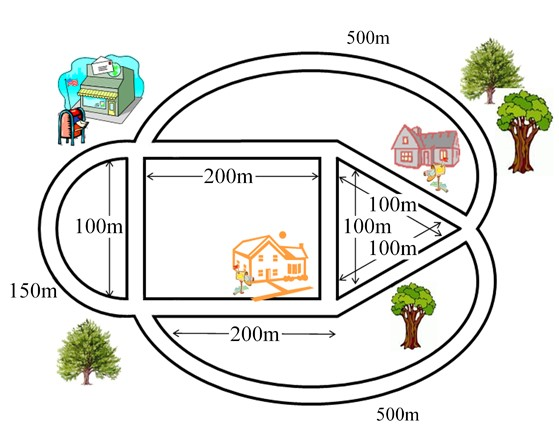
\includegraphics[scale=0.5]{Figuras/carteiro.jpg}

\end{ftst}

%=====

\begin{ftst}{História}{Ciclo Hamiltoniano}
\vone
\vone
\begin{minipage}{.5\textwidth}
\footnotesize
    O ciclo hamiltoniano recebeu o nome de Sir William Rowan Hamilton que, em 1857, inventou um jogo de quebra-cabeça que envolvia a caça a um ciclo hamiltoniano. 
    \vone
    O jogo, chamado de jogo Icosian, foi distribuído como um grafo dodecaedro com um buraco em cada vértice. Para resolver o quebra-cabeça ou vencer o jogo, era preciso usar estacas e cordas para encontrar o ciclo hamiltoniano - um circuito fechado que visitava todos os buracos exatamente uma vez.
\end{minipage}
\hfill
\begin{minipage}{.5\textwidth}
    \centering
    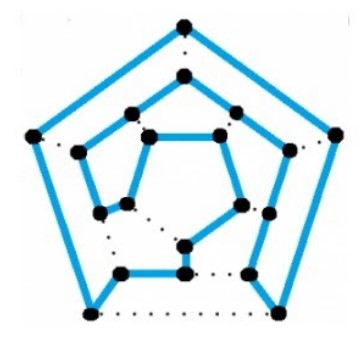
\includegraphics[scale=0.5]{Figuras/ciclo_hamiltoniano.jpg}
\end{minipage}

\end{ftst}

%=====

\begin{ftst}{Definições}{Caminho Hamiltoniano}
\vone
\vone
\begin{itemize}
    \item Um \textbf{caminho hamiltoniano} é um caminho que passa exatamente uma vez por cada vértice de um grafo;
    \item Um \textbf{ciclo hamiltoniano} é um caminho hamiltoniano fechado, ou seja, começa e termina no mesmo vértice;
    \item Um \textbf{grafo hamiltoniano} é um grafo que contém um ciclo hamiltoniano.
\end{itemize}

\end{ftst}

%=====

\begin{ftst}{Grafo hamiltoniano}{Caminho Hamiltoniano}
\vone
Não existe uma regra para determinar se um grafo é hamiltoniano!
\vone
\centering


\tikzset{every picture/.style={line width=0.75pt}} %set default line width to 0.75pt        

\begin{tikzpicture}[x=0.75pt,y=0.75pt,yscale=-1,xscale=1]
%uncomment if require: \path (0,163); %set diagram left start at 0, and has height of 163

%Curve Lines [id:da7683292464406222] 
\draw [color={rgb, 255:red, 15; green, 118; blue, 237 }  ,draw opacity=1 ][line width=1.5]    (36.33,57.67) .. controls (45.1,8.34) and (166.1,11.34) .. (179.74,57.67) ;
%Straight Lines [id:da08884414649664008] 
\draw [color={rgb, 255:red, 15; green, 118; blue, 237 }  ,draw opacity=1 ][line width=1.5]    (36.33,58.67) -- (70.33,129.67) ;
%Straight Lines [id:da48325776435904766] 
\draw [color={rgb, 255:red, 15; green, 118; blue, 237 }  ,draw opacity=1 ][line width=1.5]    (70.33,129.67) -- (107.33,58.67) ;
%Straight Lines [id:da5108779557079501] 
\draw [color={rgb, 255:red, 15; green, 118; blue, 237 }  ,draw opacity=1 ][line width=1.5]    (144.33,130.67) -- (107.33,58.67) ;
%Straight Lines [id:da42357082617222597] 
\draw [color={rgb, 255:red, 15; green, 118; blue, 237 }  ,draw opacity=1 ][line width=1.5]    (144.33,130.67) -- (215.33,130.67) ;
%Straight Lines [id:da07152389857292141] 
\draw [color={rgb, 255:red, 15; green, 118; blue, 237 }  ,draw opacity=1 ][line width=1.5]    (215.33,130.67) -- (251.33,58.67) ;
%Straight Lines [id:da7119953651174364] 
\draw [color={rgb, 255:red, 15; green, 118; blue, 237 }  ,draw opacity=1 ][line width=1.5]    (179.74,57.67) -- (251.33,57.67) ;
%Shape: Ellipse [id:dp5075093592027435] 
\draw  [draw opacity=0][fill={rgb, 255:red, 15; green, 118; blue, 237 }  ,fill opacity=1 ] (28.92,57.67) .. controls (28.92,53.66) and (32.24,50.41) .. (36.33,50.41) .. controls (40.42,50.41) and (43.74,53.66) .. (43.74,57.67) .. controls (43.74,61.69) and (40.42,64.94) .. (36.33,64.94) .. controls (32.24,64.94) and (28.92,61.69) .. (28.92,57.67) -- cycle ;
%Shape: Ellipse [id:dp13603931445795947] 
\draw  [draw opacity=0][fill={rgb, 255:red, 15; green, 118; blue, 237 }  ,fill opacity=1 ] (99.92,57.67) .. controls (99.92,53.66) and (103.24,50.41) .. (107.33,50.41) .. controls (111.42,50.41) and (114.74,53.66) .. (114.74,57.67) .. controls (114.74,61.69) and (111.42,64.94) .. (107.33,64.94) .. controls (103.24,64.94) and (99.92,61.69) .. (99.92,57.67) -- cycle ;
%Shape: Ellipse [id:dp7516959175994735] 
\draw  [draw opacity=0][fill={rgb, 255:red, 15; green, 118; blue, 237 }  ,fill opacity=1 ] (172.33,57.67) .. controls (172.33,53.66) and (175.65,50.41) .. (179.74,50.41) .. controls (183.83,50.41) and (187.15,53.66) .. (187.15,57.67) .. controls (187.15,61.69) and (183.83,64.94) .. (179.74,64.94) .. controls (175.65,64.94) and (172.33,61.69) .. (172.33,57.67) -- cycle ;
%Shape: Ellipse [id:dp9678063492720343] 
\draw  [draw opacity=0][fill={rgb, 255:red, 15; green, 118; blue, 237 }  ,fill opacity=1 ] (243.92,57.67) .. controls (243.92,53.66) and (247.24,50.41) .. (251.33,50.41) .. controls (255.42,50.41) and (258.74,53.66) .. (258.74,57.67) .. controls (258.74,61.69) and (255.42,64.94) .. (251.33,64.94) .. controls (247.24,64.94) and (243.92,61.69) .. (243.92,57.67) -- cycle ;
%Shape: Ellipse [id:dp9669459656751889] 
\draw  [draw opacity=0][fill={rgb, 255:red, 15; green, 118; blue, 237 }  ,fill opacity=1 ] (62.92,128.67) .. controls (62.92,124.66) and (66.24,121.41) .. (70.33,121.41) .. controls (74.42,121.41) and (77.74,124.66) .. (77.74,128.67) .. controls (77.74,132.69) and (74.42,135.94) .. (70.33,135.94) .. controls (66.24,135.94) and (62.92,132.69) .. (62.92,128.67) -- cycle ;
%Shape: Ellipse [id:dp9141299370953122] 
\draw  [draw opacity=0][fill={rgb, 255:red, 15; green, 118; blue, 237 }  ,fill opacity=1 ] (136.92,129.67) .. controls (136.92,125.66) and (140.24,122.41) .. (144.33,122.41) .. controls (148.42,122.41) and (151.74,125.66) .. (151.74,129.67) .. controls (151.74,133.69) and (148.42,136.94) .. (144.33,136.94) .. controls (140.24,136.94) and (136.92,133.69) .. (136.92,129.67) -- cycle ;
%Shape: Ellipse [id:dp5433101163289387] 
\draw  [draw opacity=0][fill={rgb, 255:red, 15; green, 118; blue, 237 }  ,fill opacity=1 ] (207.92,129.67) .. controls (207.92,125.66) and (211.24,122.41) .. (215.33,122.41) .. controls (219.42,122.41) and (222.74,125.66) .. (222.74,129.67) .. controls (222.74,133.69) and (219.42,136.94) .. (215.33,136.94) .. controls (211.24,136.94) and (207.92,133.69) .. (207.92,129.67) -- cycle ;
%Straight Lines [id:da21140953542973562] 
\draw [color={rgb, 255:red, 15; green, 118; blue, 237 }  ,draw opacity=1 ][line width=1.5]    (36.33,58.67) -- (144.33,130.67) ;
%Straight Lines [id:da4547447000051603] 
\draw [color={rgb, 255:red, 15; green, 118; blue, 237 }  ,draw opacity=1 ][line width=1.5]    (36.33,57.67) -- (107.33,57.67) ;
%Straight Lines [id:da9169893513605827] 
\draw [color={rgb, 255:red, 15; green, 118; blue, 237 }  ,draw opacity=1 ][line width=1.5]    (107.33,57.67) -- (179.74,57.67) ;
%Straight Lines [id:da8670329719288252] 
\draw [color={rgb, 255:red, 15; green, 118; blue, 237 }  ,draw opacity=1 ][line width=1.5]    (144.33,130.67) -- (179.74,58.67) ;
%Curve Lines [id:da030458729127779582] 
\draw [color={rgb, 255:red, 245; green, 166; blue, 35 }  ,draw opacity=1 ][line width=1.5]  [dash pattern={on 1.69pt off 2.76pt}]  (26.26,37.55) .. controls (31.35,15.22) and (76.61,11.35) .. (120.1,12.34) .. controls (164.1,13.34) and (176.1,31.34) .. (182.1,45.34) .. controls (188.1,59.34) and (249.88,34.55) .. (264.1,47.34) .. controls (278.33,60.13) and (240.1,133.34) .. (223.1,140.34) .. controls (206.1,147.34) and (159.61,138.4) .. (146.1,142.34) .. controls (132.6,146.28) and (114.1,71.34) .. (107.1,74.34) .. controls (100.1,77.34) and (88.42,142.28) .. (68.1,142.34) .. controls (49.11,142.4) and (36.78,95.14) .. (33.63,75.1) ;
\draw [shift={(33.1,71.34)}, rotate = 443.29] [fill={rgb, 255:red, 245; green, 166; blue, 35 }  ,fill opacity=1 ][line width=0.08]  [draw opacity=0] (13.4,-6.43) -- (0,0) -- (13.4,6.44) -- (8.9,0) -- cycle    ;
\draw [shift={(26.92,35.34)}, rotate = 460.31] [fill={rgb, 255:red, 245; green, 166; blue, 35 }  ,fill opacity=1 ][line width=0.08]  [draw opacity=0] (13.4,-6.43) -- (0,0) -- (13.4,6.44) -- (8.9,0) -- cycle    ;

% Text Node
\draw (14.43,52.78) node [anchor=north west][inner sep=0.75pt]    {$v_{1}$};
% Text Node
\draw (63.5,95.05) node [anchor=north west][inner sep=0.75pt]    {$v_{2}$};
% Text Node
\draw (100.18,30.8) node [anchor=north west][inner sep=0.75pt]    {$v_{3}$};
% Text Node
\draw (153.16,57.62) node [anchor=north west][inner sep=0.75pt]    {$v_{4}$};
% Text Node
\draw (225.09,58.42) node [anchor=north west][inner sep=0.75pt]    {$v_{5}$};
% Text Node
\draw (196.33,110.15) node [anchor=north west][inner sep=0.75pt]    {$v_{6}$};
% Text Node
\draw (138.33,99.15) node [anchor=north west][inner sep=0.75pt]    {$v_{7}$};


\end{tikzpicture}


\end{ftst}

%=====

\begin{ftst}{Problema hamiltoniano: caixeiro viajante }{Caminho Hamiltoniano}

Dada uma lista de cidades e as distâncias entre cada par de cidades, qual é o caminho mais curto possível que visita cada cidade uma única vez e retorna a cidade de origem?

\vone
\centering
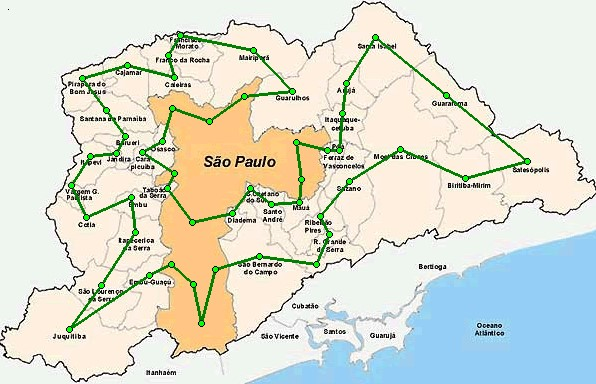
\includegraphics[scale=0.5]{Figuras/caixeiro.jpg}

\end{ftst}

%=====


\end{document}